To model each possible task that is possible in our system we used ConcurTaskTrees (CTT). These were then further used in the development of the prototype.\\
Below in figure \ref{fig:cttTop} you can find the top level of the CTT. Attached to this document you can find each image as well as a global CTT.

\begin{figure}[H]
\centering
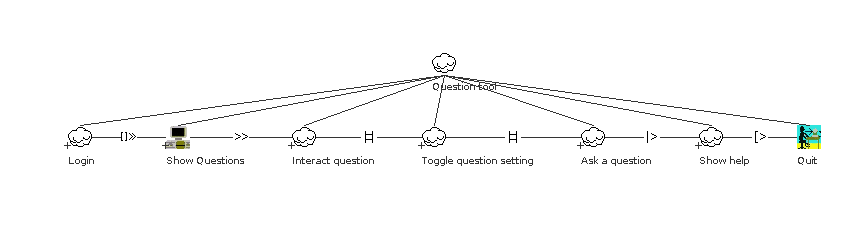
\includegraphics[scale=0.5]{../../ctt/ctttoplevel.png}
\caption{Top level CTT.}
\label{fig:cttTop}
\end{figure}
As seen there are 7 top level tasks. Before a user can do anything in our system, the user has to login. When the login is successful the users email will be passed on to the other tasks. When the login is successful the questions will be showed. Then all other tasks will be enabled. A user can stop using the application at any time which is modelled by the \emph{quit} task.\\
We will now discuss each task individually.\\

In figure \ref{fig:ctt1} CTT you can see the login task.
\begin{figure}[H]
\centering
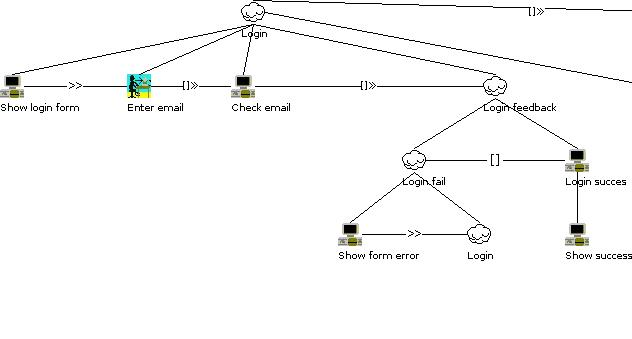
\includegraphics[scale=0.47]{../../ctt/ctt1.jpg}
\caption{Login CTT.}
\label{fig:ctt1}
\end{figure}
First the login form is displayed. The user should then provide his email address, which is then checked. Upon success the user gets a success message. Upon failure, the error is displayed on the login form and the user can try to correct this error and try to submit his or hers information again.\\

In figure \ref{fig:ctt2} the showing of questions, which happens after a user is logged in.
\begin{figure}[H]
\centering
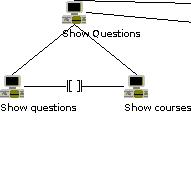
\includegraphics[scale=0.6]{../../ctt/ctt2.jpg}
\caption{Show questions CTT.}
\label{fig:ctt2}
\end{figure}
The showing of all questions is a combination of showing all courses and showing all questions. A user can then select a different course if necessary.\\

In figure \ref{fig:ctt3} the interaction with questions is modelled.
\begin{figure}[H]
\centering
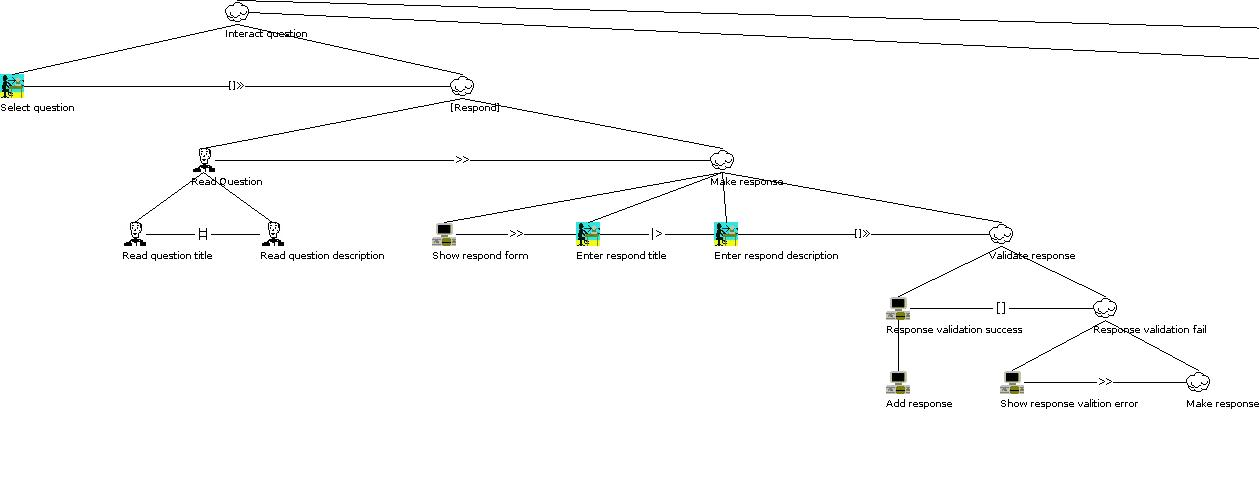
\includegraphics[scale=0.3]{../../ctt/ctt3.jpg}
\caption{Interact CTT.}
\label{fig:ctt3}
\end{figure}
A user can choose to select a question. This question (title and description) can then be read. A user can reply to a question by filling out the form (title and description), this form is then validated and the response is then posted. \\

In figure \ref{fig:ctt4} the toggling of settings. Two settings are available: the option to open or close a question and the option to make a question private or public. Private questions are only visible for the teacher and the asking user.
\begin{figure}[H]
\centering
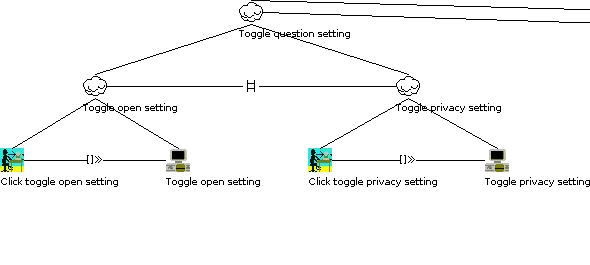
\includegraphics[scale=0.53]{../../ctt/ctt4.jpg}
\caption{Toggle settings CTT.}
\label{fig:ctt4}
\end{figure}
These toggles should be rather simple. A simple click (or similar interaction) should be enough.\\

The figure \ref{fig:ctt5} models the task of asking a question.
\begin{figure}[H]
\centering
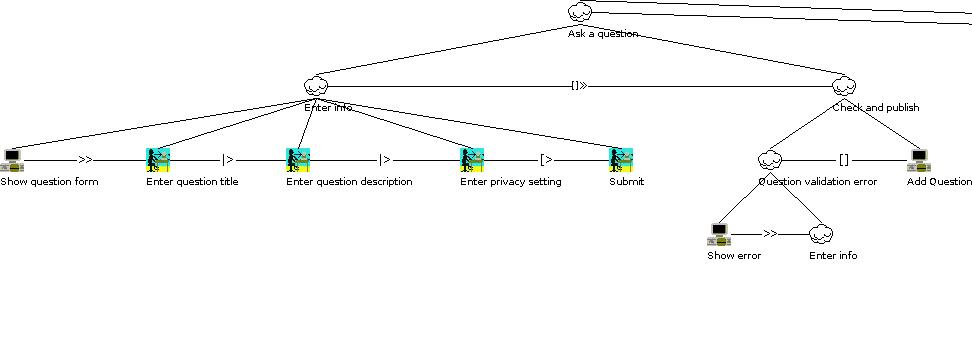
\includegraphics[scale=0.43]{../../ctt/ctt5.jpg}
\caption{Toggle CTT.}
\label{fig:ctt5}
\end{figure}
Asking a question is just a matter of showing the new question form, filling in the necessary information (title, description and whether or not this question should private then validating this form (same as for the other forms above).\\

To provide a help to users, the showing of an help overlay is modelled in figure \ref{fig:ctt6}.
\begin{figure}[H]
\centering
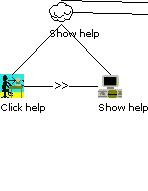
\includegraphics[scale=0.53]{../../ctt/ctt6.jpg}
\caption{Help CTT.}
\label{fig:ctt6}
\end{figure}
This can be done in a suspend-resume fashion from any of the other tasks, with the exception of the login. The user should should to open the help, after which it is displayed.

